% Copyright (c) 2014,2016  Casper Ti. Vecto 
\chapter{系统概要设计} 


	本论文提出比特币的交易监督系统(Bitcoin Transaction Monitoring System,BTMS)\supercite{Blockchain-basedpaymentcollectionsupervisionsystemusingpervasiveBitcoindigitalwallet},以下简称BTMS,BTMS以加密货币比特币实作,BTMS包含三个子系统,商家和商品信息管理子系统(Store and Merchandise Information Management Sub-System,SMIMSS)、商家手持移动装置收款及交易子系统(Store Mobile payment Collection and Transaction Sub-System,SMCTSS)、客户端行动支付和交易子系统(Client Mobile Payment and Transaction Sub-System,CMPTSS),图\ref{model0}为主系统与子系统的功能模块图。

	\begin{figure}[!htb]
		\centering
		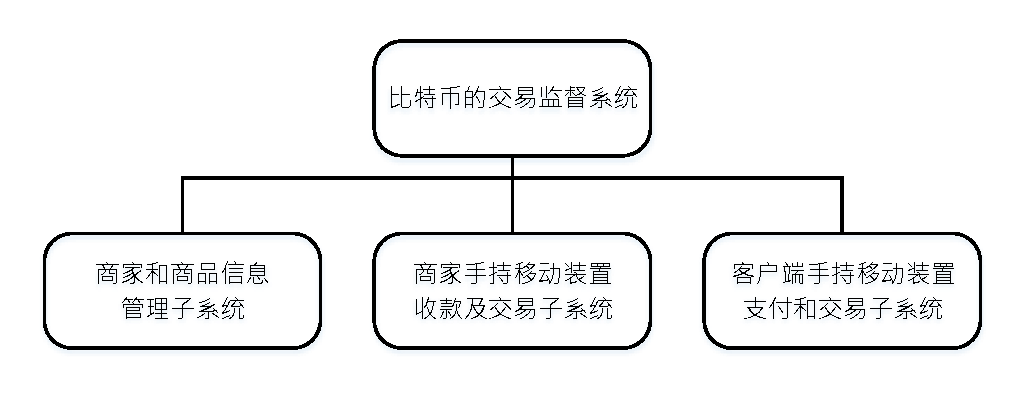
\includegraphics[width = 0.8\textwidth]{model0.pdf}
		\caption{BTMS系统功能模块图}\label{model0}
	\end{figure}

	本论文设计让商家能够结合商品与RFID标签,以达到快速建构与管理商品数据库之系统,并且让商家及顾客可以运用手持移动装置上的NFC功能来实际运作比特币的行动支付流程。商家只需要扫描商品上的RFID标签,即可快速创建交易清单,再利用NFC功能与顾客之行动设备进行信息交换,轻松地将商家的收款地址以及交易数据发送给顾客,收到数据后便能快速地以顾客之比特币行动电子钱包付款,并将交易细项保存下来,以便未来商家与顾客能够快速查找比特币行动支付的交易记录。
	本系统主要是以完成区块链之加密货币的收款监督系统为主要目标,本论文进而将积极利用自由软件的利基:使用成本低、进入门槛低、开放源代码、社区能力强、共通性及移植性强、资通安全性高等优势来开发本论文收款监督系统的应用服务平台。本系统范围包含建置下各项子系统如下:
		\begin{enumerate}
		\item 商家和商品信息管理子系统(Store and Merchandise Information Management Sub-System,SMIMSS):本系统可以让商家在进货时,快速地将RFID标签之识别码与进货商品信息集成在一起,并且透过本系统添加、修改或删除数据库内部的信息,包括产品名称、详细信息,存货数量等信息,商家与顾客便可依照该数据库取得当前商品信息与状态。不仅让商家的存货信息更加清楚明了,也可以提供顾客更多的即时服务,图\ref{model1}所示。

			\begin{figure}[!htb]
			\centering
			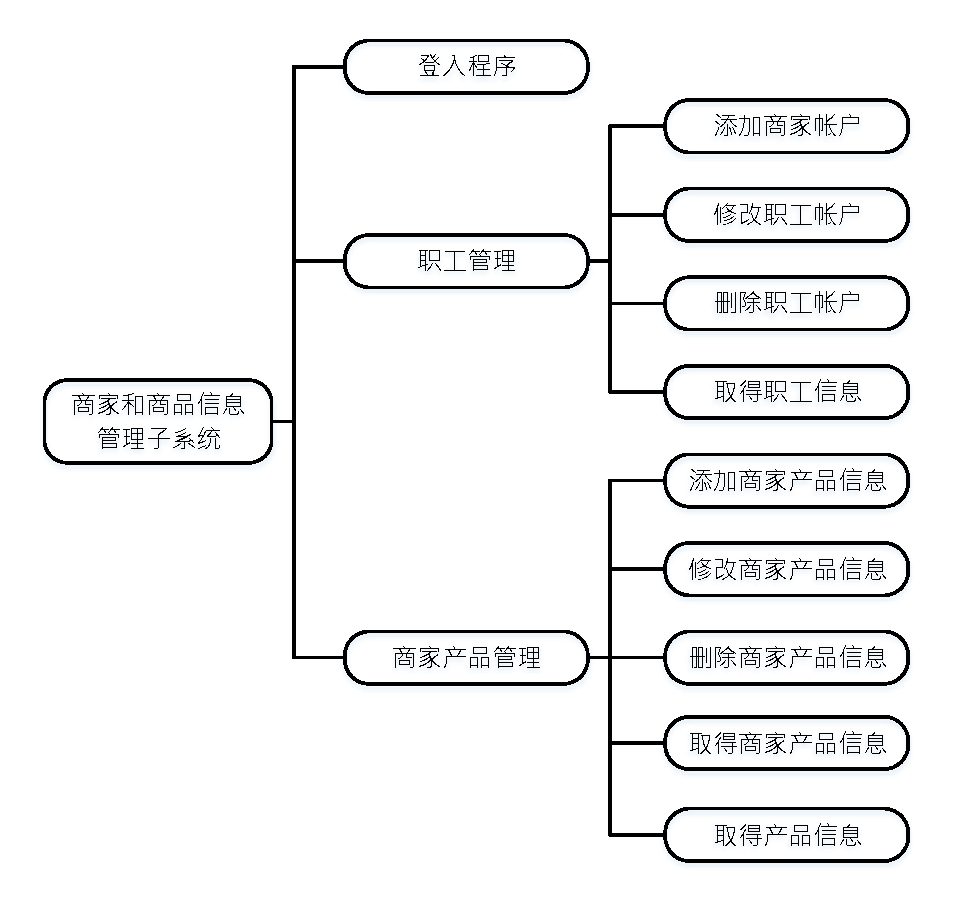
\includegraphics[width = 0.7\textwidth]{model1.pdf}
			\caption{商家和商品信息管理子系统功能模块图}\label{model1}
			\end{figure}



		\item 商家手持移动装置收款及交易子系统(Store Mobile payment Collection and Transaction Sub-System,SMCTSS):本系统使商家在结帐时,能够以手持移动装置上的NFC功能扫描商品上的RFID 标签,即可简单地创建交易清单,并透过NFC与顾客手持移动装置碰触,将交易清单以及商家之比特币收款地址等等重要交易信息一并传递给顾客,可以减短结帐的速度,使结帐效率大幅提升,其功能模块图如图\ref{model2}所示。
		 
			\begin{figure}[!htb]
			\centering
			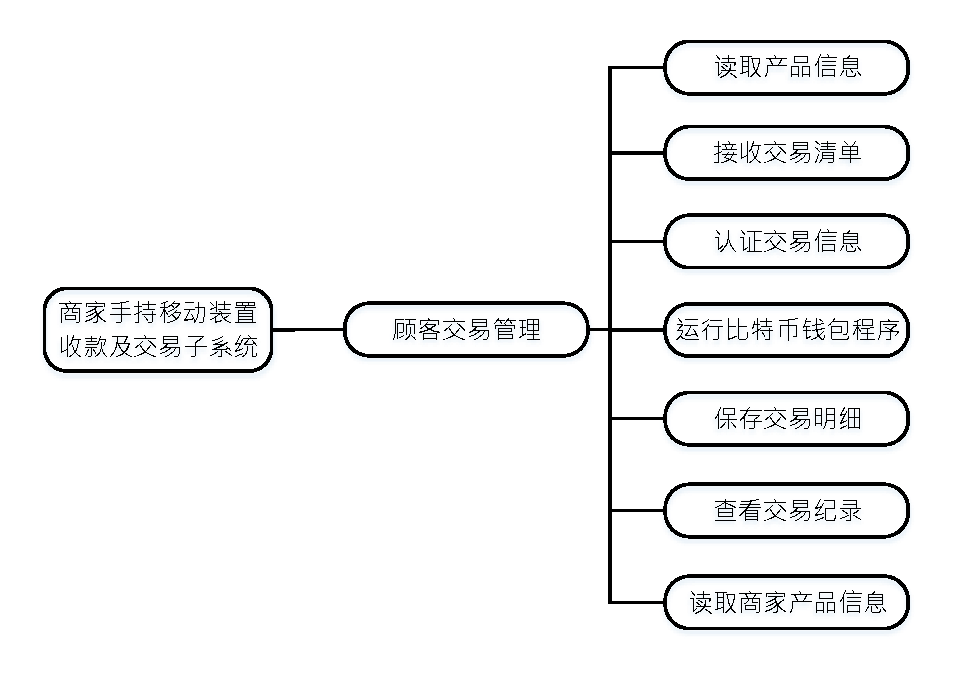
\includegraphics[width = 0.7\textwidth]{model2.pdf}
			\caption{商家手持移动装置收款及交易子系统功能模块图}\label{model2}
			\end{figure}


		\item 客户端行动支付和交易子系统(Client Mobile Payment and Transaction Sub-System,CMPTSS):顾客在结帐时,不必再麻烦的拿出信用卡或是零钱包,只需要拿出手持移动装置让职工以NFC将交易清单与比特币地址转送给自己,即可自动连接至比特币电子钱包的应用程序当中,并且自动填妥相关数据,如:交易金额、收款地址等等,与此同时也能将交易纪录保存于客户端,以便日后顾客快速取得过往的交易纪录,除此之外亦可让广大的民众体验加密货币与行动支付带来的便利生活,其功能模块图如图\ref{model3}所示。
			\begin{figure}[!htb]
			\centering
			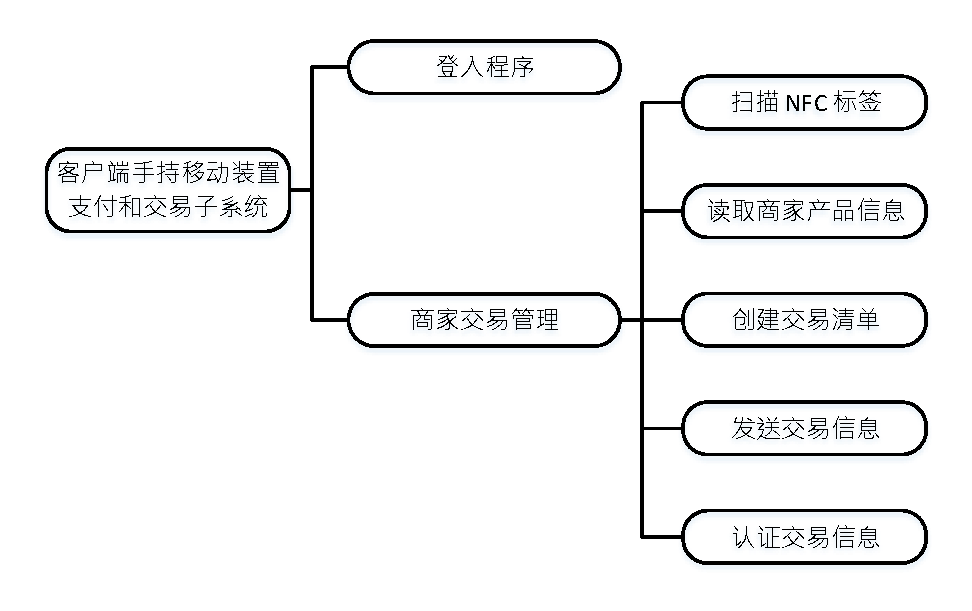
\includegraphics[width = 0.7\textwidth]{model3.pdf}
			\caption{客户端行动支付和交易子系统功能模块图}\label{model3}
			\end{figure}
		
	\end{enumerate}
	

\section{BTMS架构与运作流程}

	图\ref{fig3}为BTMS和商家注册流程架构图,商家首先需要在以下4 个步骤中完成⽤户注册与登⼊:

	\begin{figure}[!htb]
		\centering
		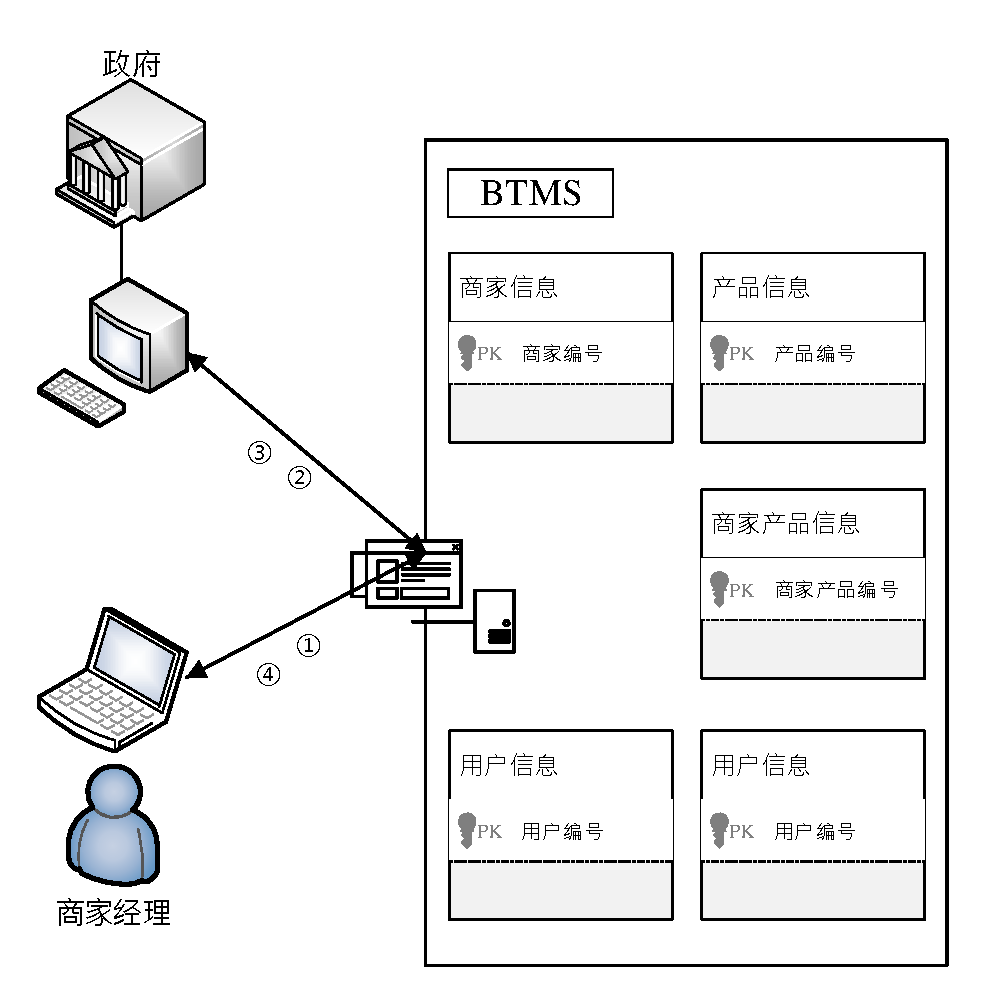
\includegraphics[width = 0.6\textwidth]{fig3.pdf}
		\caption{BTMS和商家注册流程架构图}\label{fig3}
	\end{figure}

	\begin{enumerate}
		\item 商家必须在BTMS注册一个用户,并附有政府法规的商业证明。
		\item 比特币的交易监督系统将自动向相应的政府金融监管机构提交商业申请,以审查该商家的加密货币交易业务。
		\item 如果政府批准商家的加密货币业务申请,服务器将激活商家在该收集监控系统中创建商家用户。
		\item 商家可以自由地登入帐户并添加商家想要出售的产品信息,亦可透过职工管理添加修改删除职工信息。
	\end{enumerate}

	具体的加密货币商家收银金流监控系统运行过程如图\ref{fig4}所示,以图\ref{fig3}所设计出的系统架构进行扩增,首先需要与区块链检视器 (Blockchain Explorer)\supercite{Blockchainexplorer:Ananalyticalprocessandinvestigationenvironmentforbitcoin}对接,而之所以该监控系统需要与区块链检视器对接是为了能够最直接的比对交易被记录的成交状况,能够达到即时性以及正确性,倘若担忧单一的区块链检视器成果,亦可以使用多家区块链检视器进行交叉参考,以避免因为一家公司的错误所带来的影响。区块链检视器的目的是为了能够快速地准确地比对该笔交易的成交,做为整笔交易提出到结算的环节之一。

	\begin{figure}[!htb]
		\centering
		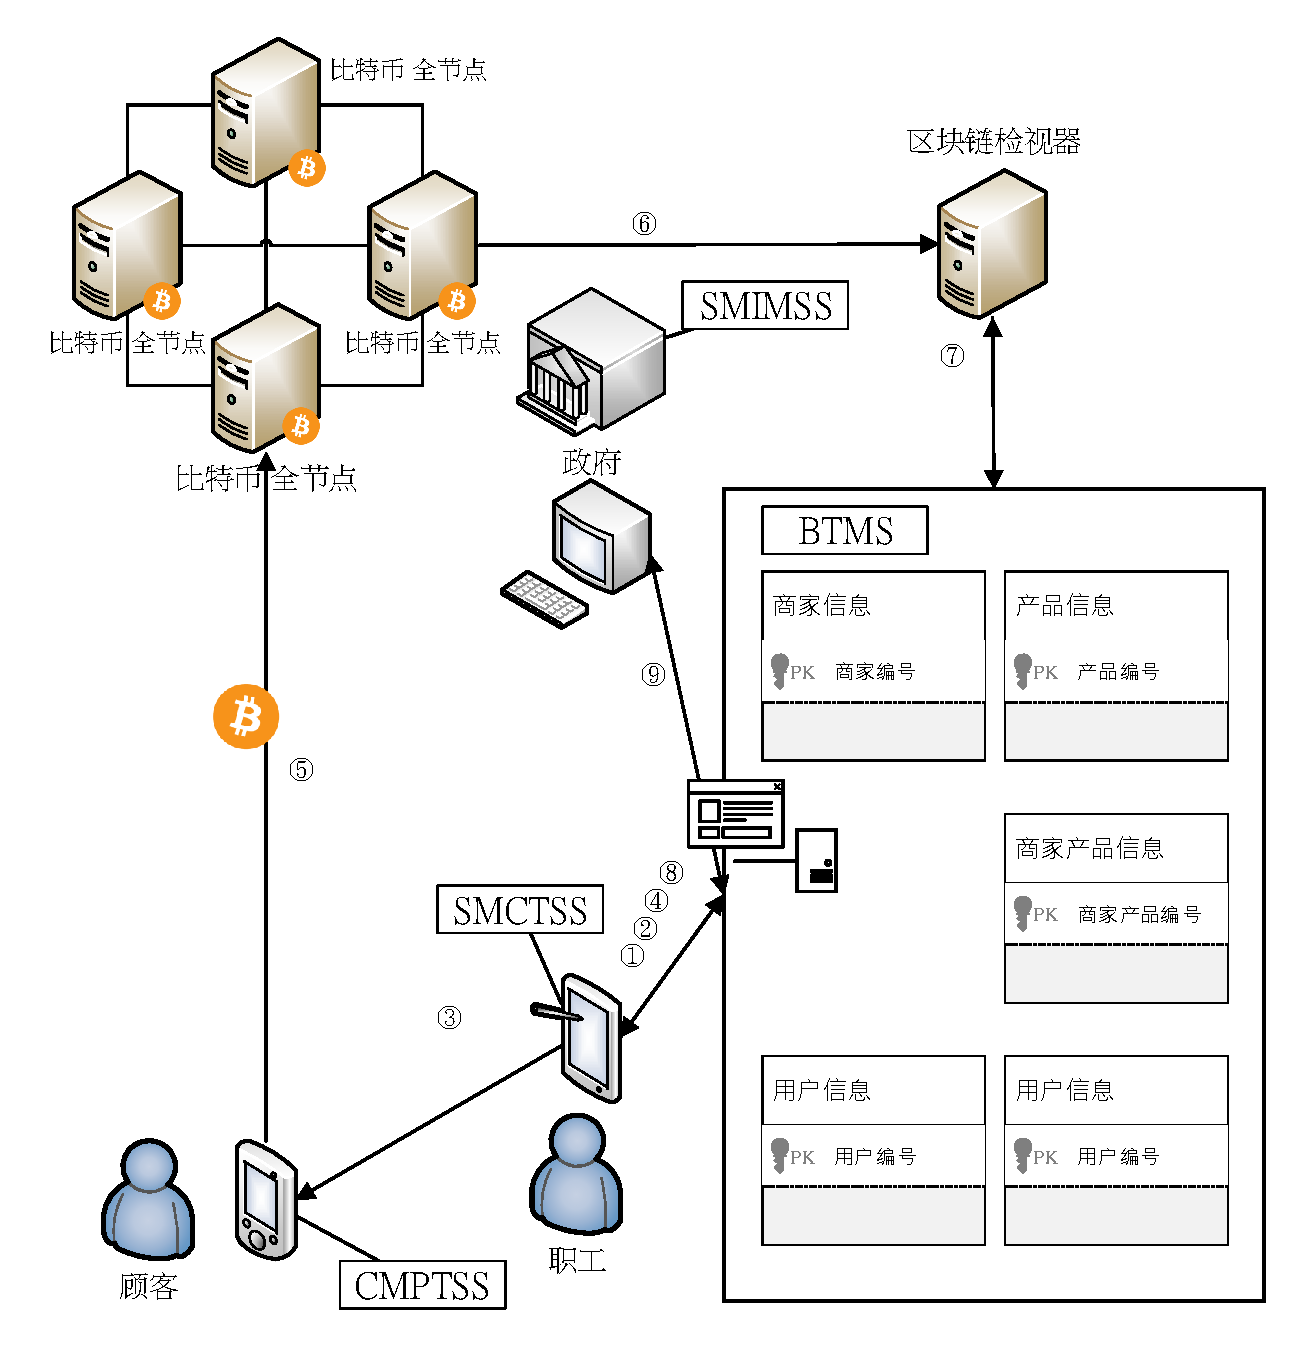
\includegraphics[width = 0.8\textwidth]{fig4.pdf}
		\caption{BTMS的整体流程架构图}\label{fig4}
	\end{figure}

	图\ref{fig4}比特币的交易监督系统创建步骤描述如下:

		\begin{enumerate}
			\item 商家职工将登入到图\ref{fig3}中的第一个步骤,完成创建用户的步骤,使用手持式平板电脑或手持移动装置访问SMCTSS中的服务。如前所述,在能够登入到系统之前,商家用户必须由政府机构审计。
			\item 在成功登入SMCTSS用于商家加密货币金流监控系统时,手持移动装置将加载通过SMIMSS注册的商家产品信息,然后创建产品目录。商家的职工可以根据顾客的需求选择所需的产品和数量。

			\item 职工使用手持移动装置完成顾客选定商品的产品信息后,手持移动装置上的NFC技术可用于将产品信息从附近职工的手持移动装置传递给顾客的手持移动装置,而无需物理交互。然后,顾客可以很容易地将自己的消费信息记录成为交易凭证等参考。在商家职⼯设备从顾客设备接收购买产品信息之后,顾客设备将向商家的手持移动装置发送其自己的比特币支付地址的信息。
			\item 商家的手持设备收到顾客确认购买所选产品的相应信息后,会将交易信息的副本发送给SMIMSS监控系统。顾客信息包括交易串行号、商家ID号码、商品号码、购买的商品数量、加密货币的收款人地址以及顾客的支付地址。
			\item 收到顾客交易信息后,即完成此次的加密货币支付。同时,此次交易的加密货币将透过客户端CMPTSS发布到比特币网络中进行验证和记录。
			\item 区块链检视器将开始分析在比特币网络中缓存池的所有交易以及区块链中记录的交易。
			\item 拟议的交易监控系统BTMS将向区块链检视器提出请求。这个请求数据不仅包括存储在BTMS中的交易副本之加密货币收款人地址,如图\ref{fig4}的第四步骤,还包括顾客预期付款的加密货币支付地址。区块链检视器使用请求数据来检查交易是否存储在区块链中,或者交易还在等待确认。如果交易已被确认并存储在区块链中,则交易数据库中校验值字段的值将更改为"1",否则其默认值为"0"。
			\item 当校验值字段中的值为"1"时,交易已完成消息可发送至商家平板电脑或⼿持移动装置上运行的商家和商品信息管理子系统(SMIMSS)。
			\item 政府财政监督部门可以审查拟议BTMS中的所有交易信息,以作为税收审计参考。
		\end{enumerate}

\section{实时BTMS架构与运作流程}

		在BTMS的机制前提下,提出比特币多重签章算法实践于政府端,将该方法称为Government Green Address,将优化后的系统称为比特币的实时交易监督系统(Bitcoin Real-time Transaction Monitoring System,BRTMS),以下则将该实时系统简称为BRTMS,BRTMS与过去Green Address 比特币钱包地址不同的在于Green Address生成需要生成两把私钥分别为用户私钥以及Green Address 机构的私钥,并将两把私钥加以合并形成Green Address钱包地址。在用户发起基于Green Address机制的比特币交易时,用户生成交易并使用数字签名,再将该笔交易发送至Green Address机构进行下一个步骤的数字签名,在这过程中完成Green Address机制交易必需依赖Green Address机构,且该机构位于海外,在封包传输上会有一定程度的延迟。为了提升国内用户可以更快速地透过多重签章技术提升交易速度,BRTMS将取代原有的Green Address机构,使得国内的用户拥有更快的网络传输速度,更快的完成多重签章算法签名。 

本节将概述本系统之商家注册、Government Green Address钱包创建与验证交易的运作流程与相关数据库架构,如图\ref{gabpcss}所示。

	\begin{figure}[!htb]
		\centering
		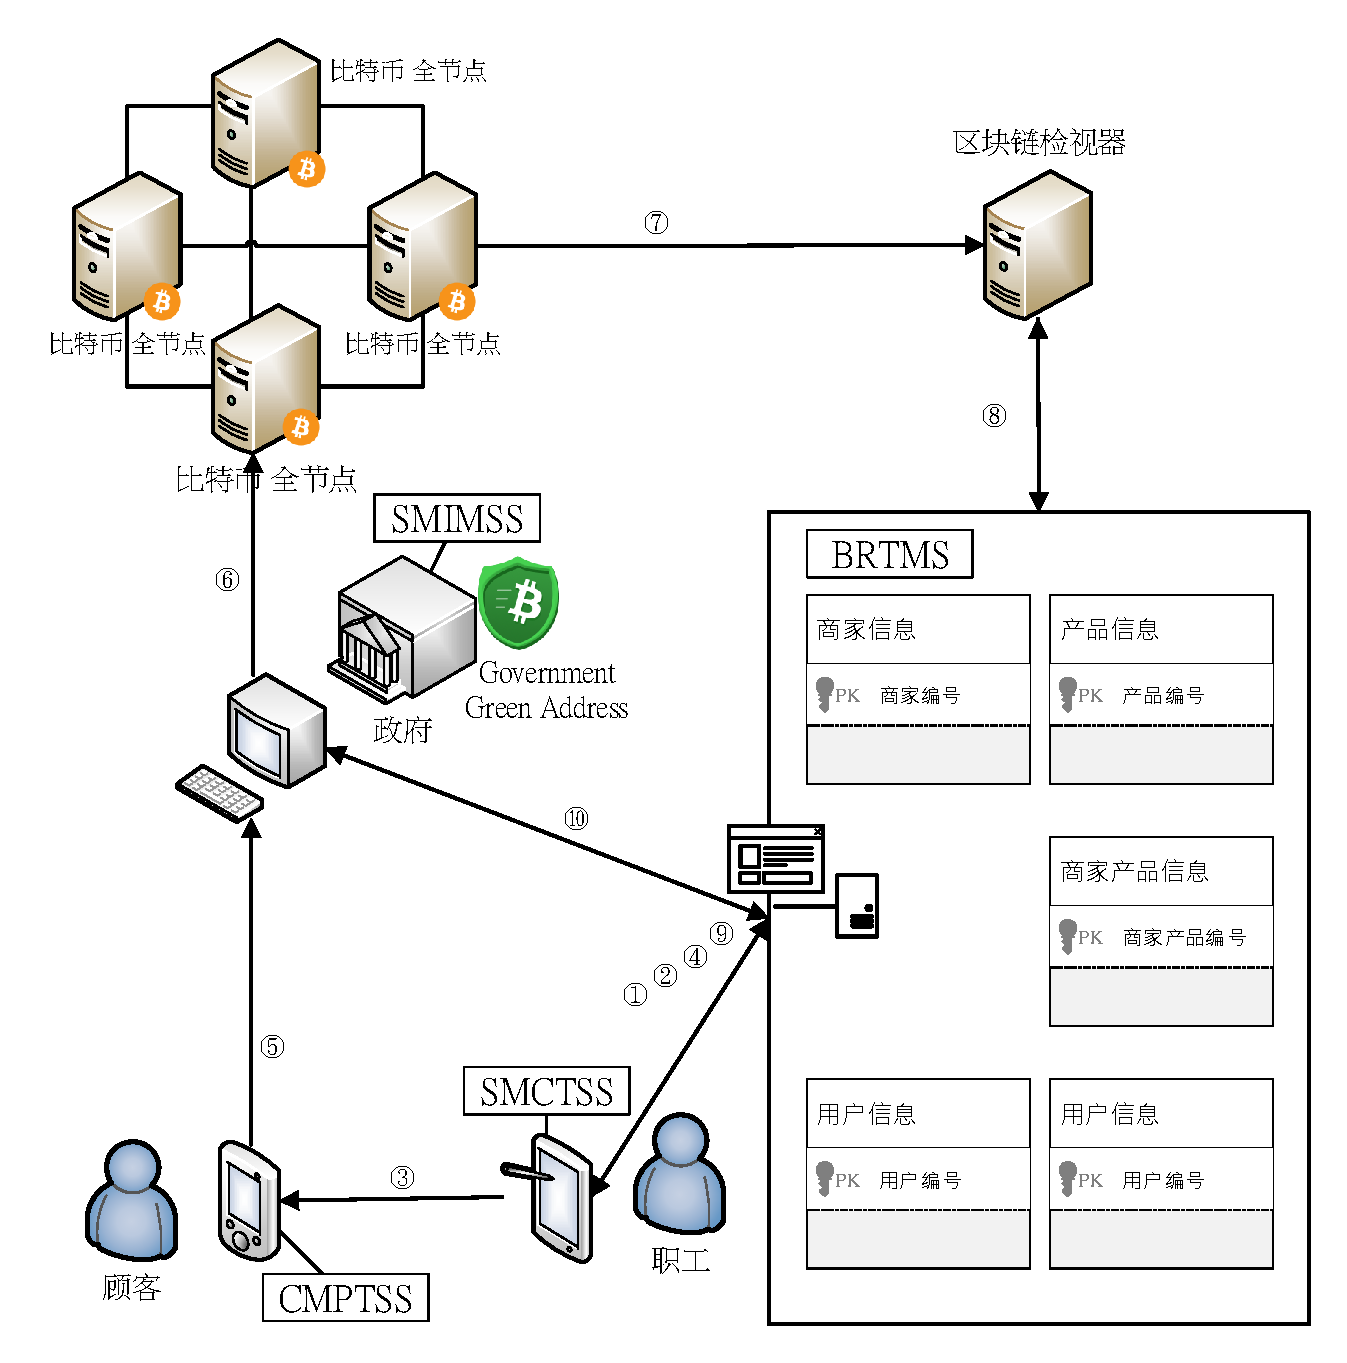
\includegraphics[width = 0.8\textwidth]{gabpcss.pdf}
		\caption{基于Government Green Address的BRTMS整体流程架构图}\label{gabpcss}
	\end{figure}

	\begin{enumerate}
		\item 商家以通过政府机构的审查审核的用户登入该系统。
		\item 系统加载该商家注册的商品信息,职工可以依照顾客的需求进行点单选取数量。
		\item 快速创建交易清单,并透过Government Green Address创建一个全新的比特币收款地址,再以Android Beam的方式将交易信息轻松地传达给顾客。
		\item 在商家职工的平板电脑收到这笔交易信息之后,会对本监督系统重送一个副本进行存盘。该交易信息包括由监督系统所提出的交易流水号、商家编号等信息。
		\item 顾客收到交易信息后,手持移动装置会自动开启Government Green Address的付款页面,确认金额无误之后便能进行支付,此时便会以顾客的比特币私钥签署交易,并等待Government Green Address机构节点的认证及发布。
		\item Government Green Address节点收到交易请求,并完成验证非双重支付攻击后,以代理节点对应地址的私钥签署本次交易,并广播至比特币节点中。
		\item 区块链检视器便会开始分析网络中所有存在缓存池中的交易,以及已经被记录到区块链中的交易。
		\item 本交易监督系统会向区块链检视器查找,检查该笔交易是否已经存在于缓存池当中,若已经确认进入缓存池,则认定该笔交易成立并完成付款。
		\item 在交易确认之后,便向商家职工的平板电脑送出交易已经成交的信息,此时完成交易,于此同时也将该笔交易信息建置于系统数据库内。
		\item 后续政府可以连入BRTMS系统查看交易信息。
	\end{enumerate}